% paper.tex
% sample ACM SIG Proceedings document using LaTeX2e
% Author: Heila van der Merwe
% based upon LaTeX2.09 Guidelines, 9 June 1996
% Revisions:  17 July 2012
%
\documentclass{sig-alternate}
\usepackage{listings}
\begin{document}


\title{Verifying Android Applications using Java PathFinder}

\numberofauthors{3}

\author{%
\alignauthor  Brink van der Merwe\\
 \affaddr{Dept. of Computer Science}\\
       \affaddr{University of Stellenbosch}\\
       \affaddr{Private Bag X1 Matieland}\\
       \affaddr{South Africa, 7602}
       \email{abvdm@gmail.com}
\alignauthor Heila van der Merwe\\
       \affaddr{Dept. of Computer Science}\\
       \affaddr{University of Stellenbosch}\\
       \affaddr{Private Bag X1 Matieland}\\
       \affaddr{South Africa, 7602}
       \email{heilamvdm@gmail.com}
\alignauthor  Willem Visser\\
 \affaddr{Dept. of Computer Science}\\
       \affaddr{University of Stellenbosch}\\
       \affaddr{Private Bag X1 Matieland}\\
       \affaddr{South Africa, 7602}
       \email{willem@gmail.com}
}


\maketitle

\begin{abstract}

\end{abstract}

% A category with the (minimum) three required fields
\category{H.4}{Information Systems Applications}{Miscellaneous}
%A category including the fourth, optional field follows...
\category{D.2.8}{Software Engineering}{Metrics}[complexity measures, performance measures]

\terms{VERIFICATION}

\keywords{Java PathFinder, JPF, Android, Verification} % NOT required for Proceedings

%The current trend in software development is mobile application development.
%At Google I/O 2012 Android claimed to have approximately 600
%thousand applications on the market with a total of 20 billion application downloads. They continue to note that this number is growing by
%one billion per month.
%Although Android mobile applications and Java desktop applications both use the Java language, they are developed for completely different
%platforms.  and both contain many similar errors and defects. These defects include faults such as concurrency issues and run-time
%exceptions. 
%are  compared to

\section{Introduction}
Software testing and verification is a crucial part of software development. It determines the quality and the user
experience of software which are two very important aspects of Android applications. Especially for the high volume Android applications
that are released. 

Although application testing is so important, it is often neglected as a result of its complex and time consuming process. Android
applications also face additional challenges when it comes to software testing:

Firstly, Android applications are graphical user interface (GUI) based. Their application flow is hence driven by GUI events. The
simplest way to test GUI applications is manual black-box testing, but this is time consuming, error prone and
expensive~\cite{AccessibilityTech}. Furthermore, user input is not the only factor that determines application flow. Android applications
also receive input from system events. These include events such as battery low and network down warnings as well as start application and
stop application commands.

Secondly, Android applications are developed in a custom implementation of Java adopted from the Apache Harmony~\cite{harmony} project. The
compiled applications can only be executed on a special virtual machine (VM) called the DalvikVM that is part of the Android operating
system~\cite{dalvik}. Hence Android applications can only run on a computer in an Android emulator. This makes testing very slow and
difficult to automate.

Due to these challenges, the rapid pace at which applications are developed and the lack of testing tools available, mobile application
testing becomes too expensive in terms of time and money. An important method to reduce this high cost, is to 
automate the testing of GUI -- in this case Android -- applications~\cite{AccessibilityTech}.

Currently, Android applications are tested automatic in one of two ways:

The most common way to test Android applications is using a physical device/emulator. Testing frameworks such as
the MonkeyRunner~\cite{monkey} and Robotium~\cite{robotium} makes use of Android's built-in JUnit framework~\cite{TestingAndroid} to
execute test on the emulator/device. Other projects use alternative ways to automatically generate input by manipulating the built in
accessibility technologies~\cite{AccessibilityTech} or by re-implementing the Android keyboard~\cite{KeyboardModel}. Mockito~\cite{mockito}
and Android Mock~\cite{androidMock} allows JUnit testing on the DalvikVM by using a mocking architecture.

The advantage of running the application on the Dalvik VM is that the application runs on the actual android operating system. The
disadvantage is, as mentioned before, Android applications are driven by user and system events. So the input has to be modelled which is
not simple to
automate on a device/emulator. Moreover running test on the Dalvik VM is slow as they have to be instrumented and each test sequence has
to be defined and executed one by one. 
 
The other approach is to test Android applications by using the Java Virtual Machine (JVM). There are different ways of implementing such a
framework. Android
lint~\cite{lint}, for example, makes use of static analysis to identify common errors in applications. Robolectric~\cite{robolectric}
intercepts the loading of Android classes and then uses shadows classes that model these classes.

Although Android applications and Java desktop applications are designed for completely different Java virtual machines, they are both
built on an implementation of the Java Application Programming Interface (API). As a consequence, Android applications contain many of the
same errors as Java applications. These defects include but is not limited to concurrency issues and runtime exceptions. It follows that it
is possible to adapt an existing testing frameworks for Java applications, to verify Android applications on the JVM.

% what are we going to do and why 
This paper describes an extension to Java PathFinder (JPF)~\cite{JPFDocs} that enables the automatic
verification of Android Applications on the standard Java JVM. 

This paper will first provide an overview of JPF and how it can be used to test Android applications. Thereafter a description of the
development of the jpf-android tool is provided, followed by a simple example to show how the tool works.


\section{Design}
\subsection{Java PathFinder}
JPF is an automated open source analysis engine for Java applications~\cite{JPFDocs}. It is implemented as explicit state model checker
that includes mechanisms to model Java class files, model native method calls (MJI), track bytecode execution and listen for
property violations. Additionally, JPF's design encourages developers to create extensions to the framework. Currently there exists many
extensions including a symbolic execution extension (jpf-symbc), data race
detector (jpf-racefinder) and an abstract window toolkit (AWT) extension (jpf-awt).

The JPF Android extension (jpf-android) will use JPF's extension mechanisms to:
\begin{enumerate}
\item model the Android library classes so that Android applications can run on the JVM
\item create an input model to simulate user and system input to the application.
\end{enumerate}

One of the advantages of extending JPF is that it has been rigorously tested and already works for Java applications. As soon as
Android applications can run on JPF, common software errors such as null pointer exceptions, assertion violations, deadlocks,
race-conditions will be detected.

The first step in modelling the android class libraries is to understand the structure of the Android operating system (OS).

\subsection{The Android operating system}

The Android OS is built on top of the Linux kernel. For security reasons, each Android application is installed as a separate user
on the OS. Linux's built-in user management system then keeps applications from modifying the data and code of other applications. For
even more security each application is run as a separate process on the OS. The applications can only interact using the Binder
inter-process communication (IPC) mechanism. The main process/application of the OS is called the system process. The system process
contains services responsible for running the main tasks of the OS for example:
\begin{itemize}
 \item activity manager -- manages the life-cycle and interaction of all the activities running in the system
 \item window manager -- allows applications to draw on the screen
 \item package manager -- stores information on the application packages installed on the device
\end{itemize}

Android follows a single-threaded application design in which a main thread handles all application events. This structure is
commonly used by many UI frameworks since it becomes too complex to make all UI classes thread safe~\cite{}. This main thread is called
the \texttt{Looper} and has a message queue attach to it containing application events to be handled. When UI events are fired, they
are added to the \texttt{Looper}'s message queue. System events are also scheduled on the main \texttt{Looper} by adding them to the message
queue. The \texttt{Looper} is responsible for continuously looping through these messages and handling them appropriately. This could
include updating a widget, loading a new activity or processing an intent.

The main class of an Android application is called the \texttt{ActivityThread}. The \texttt{ActivityThread} keeps track of the
application's components and handles user and system events. Android applications written by developers consists of the
following application components:
\begin{itemize}
\item Activities -- responsible for representing and managing an user interface. An application can consist of many
Activities.
\item Services -- performs background operations such as the pulling of messages from a server every 5 minutes. Services do not have user
interfaces and an application can have zero or more services running simultaneously.
\item Broadcast receivers -- listens for and responds to system-wide events such as network failing, low battery or screen orientation
change events.
\item Content providers -- manages application data stored on the file system, in databases, on the web or other storage medium and provides
a gateway to this data from other applications.
\end{itemize}

These components are created and managed by the \texttt{ActivityThread}.They interact with each other and with other
applications using a structure called an \texttt{Intent}. An \texttt{Intent} is a high level implementation of the Binder IPC.

\subsection{Scope of jpf-android}
The Android platform is very large and one of the main challenges is to decide which parts of the system to model. The objective of
jpf-android is to test Android application not to model the Android framework, so we do not necessarily want to model the entire
Android OS. Additionally, the more of the framework is modelled, the more has to be re-modelled when Google changes the design.

jpf-android will only model one application with multiple components and their interaction. Furthermore the graphics libraries will not
be modelled as we do not have to physically draw on the screen for testing. The system service of the Android OS is not run in the
application process and runs in its own thread. To reduce scheduling possibilities we will not model this service, but implement the
necessary tasks as part of the application process. Lastly, as the application will not be communicating with outside processes, the Binder
IPC will not be modelled. The components will communicate with each other by sending direct references to themselves. 

\section{Development}
At the basis of the tool's modelled framework are the message queue, the view structure and the activity manager. These components will be
discussed in greater detail below:

In the Android framework all input events of the system are placed on the message queue and then processed by the \texttt{Looper}. Hence,
jpf-android needed a way to place events in this queue. jpf-awt introduced the idea of using a simple script to write event sequences as
input for the application. This scripting mechanism made use of JPF's state backtracking feature to support elements such as the ANY and
REPEAT structures to make it simpler to specify many input sequences simultaneously. Each time the message queue is empty an event is
read from the script file. 

As Android and AWT both use a single-threaded UI design, jpf-android could build on the idea of scripting input events. There were two
challenges to using this approach in jpf-android:
\begin{enumerate}
 \item Android applications other that AWT applications receive input from two different
sources: user input from the UI, and system input from the activity manager through Intents. 
 \item Android applications contains multiple windows - one for each Activity. This complicates the UI input as each
window has its own unique set of view components - thus a unique input sequence.
\end{enumerate}
These challenges were addressed by expanded the scripting language in a few ways:

\subsection{The input model}
jpf-android classifies input events as either UI events or system events. UI events are handled similar to
how they were handled in jpf-awt. When the activity's UI is inflated, an object map is built binding the name of a view component (widget)
to a reference of the inflated view object. When an UI event occurs the name of the target view component is looked-up in the object map
and then the action is called on the actual view object. 

An Intent-object are used to describe system events. Intents are used to start Activities
and Services or to provide a notification of certain events. They are similar to messages containing a description of an operation to be
performed or, often in the case of broadcasts, a description of something that has happened and is being announced. The are two types of
Intents:
\begin{itemize}
 \item explicit intents -- explicitly store the name of the component to start
 \item implicit intents -- store the details of a event that occurred these details are then used to lookup components that are registered
for such events. Component's register for intents in the AndroidManifest file. Now to resolve the component to which the intent is sent an
the ActivityManager has to parse the AndroidManifest file. This file contains the the list of Intent filters for each
Application component. 
\end{itemize}

But the ActivityManager requires information about which component to send the intent to: an Activity, Service or Receiver. In the Android
code
an Intent is sent by calling one of the methods \texttt{startActivity(Intent), startService(Intent), sendBroadcast(Intent)}. Usually this
request is sent to the activity manager where it is handled appropriately. But as we are not modelling the
ActivityManger, the Intent is handled by a local, small model of the ActivityManager. The Activity Manager then resolves the intent to the
appropriate application and then forwards the intent to the application's ActivityThread to be processed.

To allow a user to script system events, variables were added to the scripting language. Variable names will be identified by
the '@' in front of the name as '\$' is already used in jpf-awt to identify UI components:

The script file that send an intent to start the \texttt{SampleActivity} will look like:
\begin{figure}
{\small
{\sf 
@intent1.setComponent(``SampleActivity'')\\
startActivity(@intent1)\\
\$button1.onClick()
}
}
\caption{Starting an Activity}
\end{figure}










\subsection{The input sequence}
jpf-android started out by using a sequential input script that drove the application execution. This became an issue when some of the
input events were non-deterministically scheduled to happen. In other words, if we do not know whether an event took place or
not, we can not schedule following events. Hence, the scriptwriter has to have knowledge of the system and
know which button press fires what activities. There could in be non-determinism in term of events but not in terms of starting
activities/services. This is because if an Activity is started, the following events in the script must be related to the new Activity. 

Lets look at an example:
\begin{figure}
\centering
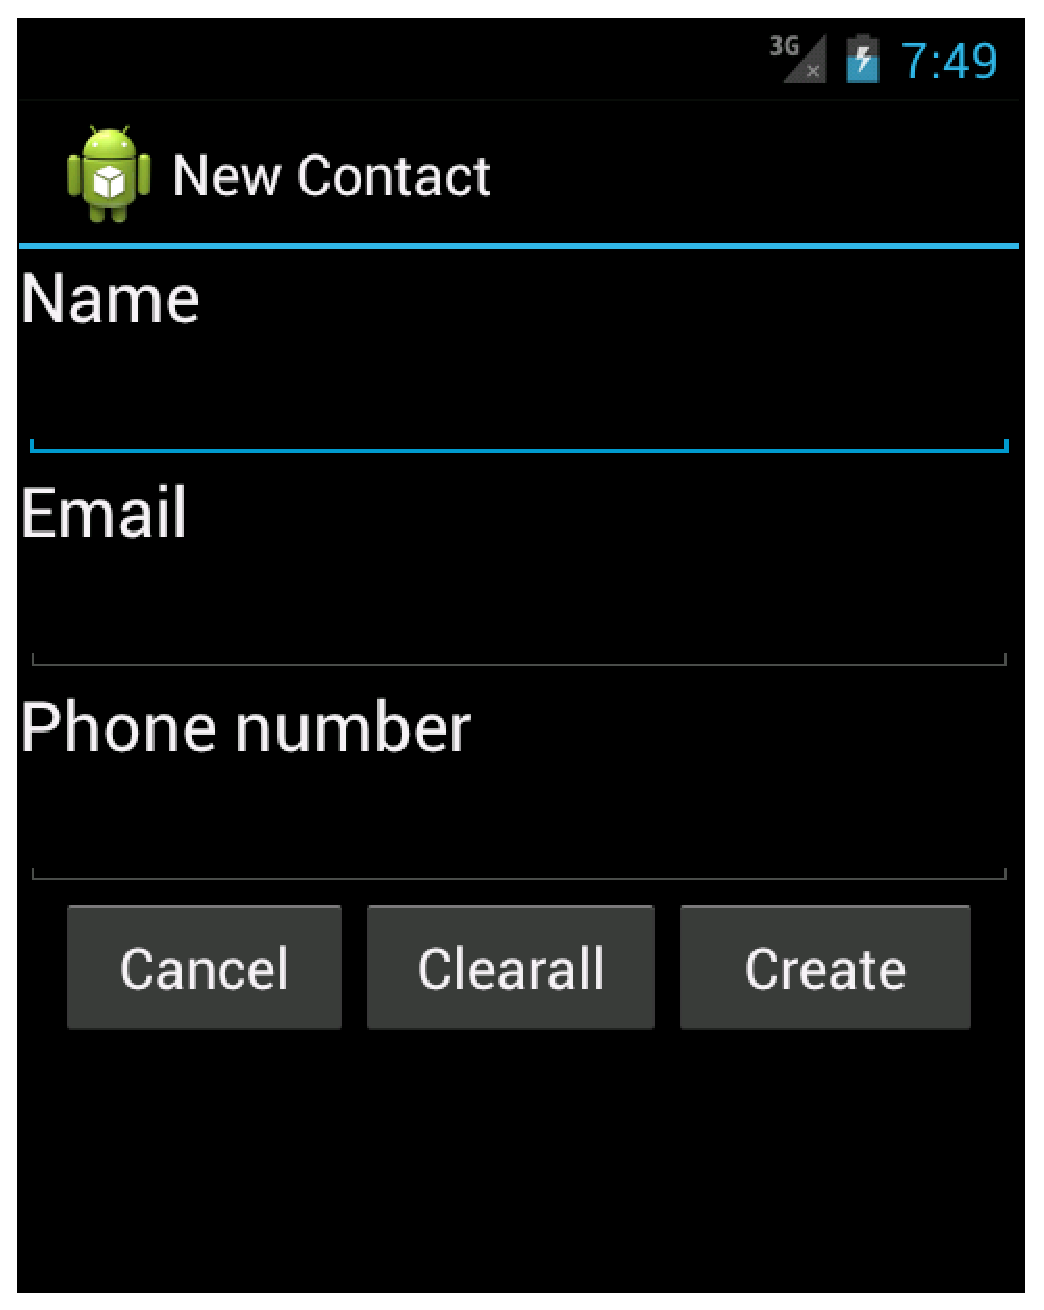
\epsfig{file=newContact.eps, width=1in,}
\caption{Adding a new contact screen}
\end{figure}

This is the Create new contact screen of a phonebook application. At the bottom of the screen there are three buttons. The cancel button
returns to the previous screen, the clear button stays on the current screen and the create button forwards to a new screen. Noe  let us
look at the following input script:

\begin{figure}
{\small
{\sf 
@startIntent.setComponent(``com.example.AddContactActivity'')\\
startActivity(@startIntent)\\
\\
\textbf{REPEAT} 3 \{\\
\textbf{ANY} \{backButton.onclick(),clearButton.onClick(),addButton.onClick()\}\\
\}

nameEdit.setText(``Mary'')
}
}
\caption{Starting an Activity}
\end{figure}

This script file will execute 3 event sequences:
\begin{enumerate}
 \item start AddContactActivity\\
press clearButton\\
set name edit's text
 \item start AddContactActivity\\ 
 press addButton button, \\
 set name edit's text
 \item start AddContactActivity\\
 press homeButton button, \\
 set name edit's text
\end{enumerate}

The problem is that only after the clear button is pressed is the nameEdit.setText(`` Mary'') command valid as we do not know if the other
screens contain textboxes.

Android applications have many Activities, each with a unique interface. At any time, the system or the UI can fire an event to start a new
Activity. The problem is as this is a nondeterministic chance the the input file can not run sequential. So that when an Activity is
started, jpf-android can go and look up what are the event sequences that can be performed on the activity.


To address this issue, we adopted the input script to be divided into sections. Each section list the sequential input to an specific
Activity:




\begin{figure}
{\small
{\sf 
@startIntent.setComponent(``com.example.ListContactsActivity'')

\textbf{TARGET:} start\\
startActivity(@startIntent)\\

\textbf{TARGET:} com.example.ListContactsActivity\\
listbox.select<0-N> \#starts ViewActivity\\

\textbf{TARGET:} com.example.ViewContactActivity\\
backButton.onClick() \# restarts ListContactsActivity, \\
   
}
}
\caption{Starting an Activity}
\end{figure}
so how do we know not to run sequence again other wise infinite loop?




The next challenge 
-  returning to an activity don't wan to execute sequence again example contacts list contact - view contact - list contact

\begin{figure}
{\small
{\sf 
TARGET: start\\
  startActivity(ListContactsActivity)

TARGET: com.example.ListContactsActivity\\
  listbox.select<0-N> \#starts ViewActivity

TARGET: com.example.ViewContactActivity\\
   backButton.onClick() \# restarts ListContactsActivity, 
}
}
\caption{Starting an Activity}
\end{figure}








The question is how do we then backtrack the case where an activity was started?

All state that is stored in the JPF side will be backtracked automatically, but we are not on the JPF side. We have to know when an
activity is started as a backtrack or as a new start. 






entrypoint 
\newpage
\section{Case Study}
% example showing the detection of a null pointer exception in certain case





\section{Discussion}
%discussion showing how the tool is successful and the advantages of the tool


limitations
- only 1 application
- no android native code can be handled

\section{Conclusion}






\section{Acknowledgements}

%
% The following two commands are all you need in the
% initial runs of your .tex file to
% produce the bibliography for the citations in your paper.
\bibliographystyle{abbrv}
\bibliography{paper}  % sigproc.bib is the name of the Bibliography in this case
% 
\end{document}
